% Document class options:
% 11pt for 11 point font
% oneside for not weird margins between odd and even pages
% (omitting oneside gives a better margin setup for print
% but i'm guessing  you're handing this in)
% a4paper to A4 page size, because LaTeX by default is setup
% to use US Letter paper size, because Donald Knuth
% the article class, as the book class is designed for
% larger documents and you probably don't need chapter
% environments
\documentclass[11pt, oneside, a4paper]{article}
\usepackage[utf8]{inputenc}
\usepackage[english]{babel}

\usepackage{hyperref}
\hypersetup{
    colorlinks=true,
    linkcolor=black,
    filecolor=magenta,      
    urlcolor=cyan,
}

\urlstyle{same}

\usepackage[utf8]{inputenc}
\usepackage{graphicx}
\usepackage{array}


% Set spacing (i set it to 1.2x)
\renewcommand{\baselinestretch}{1}
% Indentation (set this to zero for normal prose)
\setlength{\parindent}{0em}
% Line breaking (spacing between paragraphs)
\setlength{\parskip}{0.5em}

% Use the whole page
\usepackage{geometry}
% Extra math glyphs
\usepackage{amsmath}
% Proper enumerate spacing
\usepackage{enumitem}
% More pleasing screen fonts
\usepackage{lmodern}
% Fancy headers
\usepackage{fancyhdr}
\usepackage{graphicx}
% Allows absolute positioning of images
\usepackage{float}
% \usepackage[section]{placeins}
% Set no separation
\setlist{noitemsep}
% Set margins to reasonable
\geometry{margin=2.5cm}
% Sets graphics path
\graphicspath{ {./images/} }
% Sets up fancy headers
\pagestyle{fancy}
\fancyhf{}
\lhead{Natalie Hong Data Visualization Project Report}
\rhead{COSC3000}

\addto\captionsenglish{
\renewcommand{\listfigurename}{List of Graphs}
}

\usepackage{listings}
\usepackage{color}

\pagestyle{plain}

\begin{document}


\definecolor{dkgreen}{rgb}{0,0.6,0}
\definecolor{gray}{rgb}{0.5,0.5,0.5}
\definecolor{mauve}{rgb}{0.58,0,0.82}

\lstset{frame=tb,
  language=Python,
  aboveskip=3mm,
  belowskip=3mm,
  showstringspaces=false,
  columns=flexible,
  basicstyle={\small\ttfamily},
  numbers=none,
  numberstyle=\tiny\color{gray},
  keywordstyle=\color{blue},
  commentstyle=\color{dkgreen},
  stringstyle=\color{mauve},
  breaklines=true,
  breakatwhitespace=true,
  tabsize=3
}

\thispagestyle{empty}

\tableofcontents

\listoffigures

\newpage

\pagenumbering{arabic}

\section{Introduction}
Super Smash Bros. Ultimate, a game for the Nintendo Switch is an immensely popular game with an amazing competitive community nationwide. This report was created with the aims of giving the Australian competitive community a better insight into character changes and skill gaps between each quarter of 2019 and differences between rising skill levels of states. This insight will be properly visualised through multiple data graphs including that of univariate, bivariate and multivariate representations.


\section{The Data Set}
Hello and welcome to my report about data visualisation. My name is Natalie and I am a third year Software Engineering student and I'm enjoying this course so far.
\

The data set I have chosen is that of character usage, skill gain and played matches revolving around that of a local competitive gaming community in Australia. The way I have chosen to present this data set is through that of local JavaScript which calls the Google Chart library. This means that I will be able to deploy a live website showing this data for later viewing and later analysis. 
\

As data is always changing in database I was using, I decided to only pull data from last year (2019) to give a more accurate representation of data and split them into each quarter (every 3 months). Since I am an active player within this community, I believe that releasing this data publically will allow for a more insightful look into the past and how the metagame (accepted norm) of the community has changed.
\

I hope that you will find this interesting even if you don't play games.

\section{Techniques, Methods and Execution}
In this section, I will talk about my approach to the data collection; how I handled the data and how I displayed the data in web form.
\subsection{Techniques - The Approach to the Data}
The data that I was trying to access was that of a public API that I could easily access through Python. 

The data was stored in JSON form which meant that I had to iterate through various levels of data to get the data that I wanted. 

Since I was on a mac, I had to create a virtual environment to be able to access the API. Once I set up this environment, I created a Python script then called the API using a variety of similar functions to the code block below.

\begin{lstlisting}    
headers = {'Content-Type': 'application/json',
           'X-ApiKey': '6PG3OWV9UCVFZNTXQJKR'}

# ID being the character ID
def character_matches(id):
    url = 'https://api.ausmash.com.au/characters/{}/matches'.format(id)
    response = requests.get(url, headers=headers)
    
    content = json.loads(response.content)
    # JSON file of the content received and returned. It can now be stored for further use.
    return content

\end{lstlisting}

Using similar functions to the above, I was able to create a large dictionary in Python which contained all my data. This structure was split into quarters, by state and then by characters, with each character containing the unique players, the amount of elo gained and the amount of matches played. How I was able to sort this data into a more readable and interactable form can be seen in the next section.

\href{https://api.ausmash.com.au/swagger/ui/index#/}{(Click for API Documentation)}

\subsection{Methods - How I Handled the Data}
Before working towards getting my data, I had decided that I wanted to pull elo gain (skill gain, it will be called elo throughout the report), the unique amount of players who played each character and the amount of matches played for the specific character. Each character's data would then be sorted into states which would then further be stored into quarters (every 3 months e.g. Q1 is from January 1st 2019 to March 31st 2019).

To do this, I iterated through every single character's logged matches and got each unique player, their state and the won elo if the player won the match. I would also get the date and would match the date to the associated quarter. Once this was done, I then added their data to a large dictionary data structure.

Once the data was fully sorted, I wrote the contents of the dictionary into a JSON file which was then to be used for my JavaScript file which would display the data using Google Charts. This JavaScript usage will be explained in the next section.

\subsection{Execution - Displaying the Data}
Using \href{https://developers.google.com/chart}{Google Charts} I was able to create various suitable graphs for my collected data using native JavaScript. The chosen graphs that were used for my data visualisation were that of:
\begin{itemize}
	\item Bar Charts
	\item Bubble Charts
	\item Line/Area Charts
	\item Scatter Plots (using the same library as Bubble Charts)
	\item Step Graphs
\end{itemize}

Order of iteration through my chosen data would change depending on which graph I had chosen and and what I wanted to display. This lead to many different variances of the same code which would each have different outcomes. For example, for some code I would need to iterate through quarters rather than the states. When running the script for my data, I also made sure to check the player's state of origin rather than where they competed to account for interstate tournaments and visits. 

When I wanted to create the specified chart, I would create an array to hold the data in it called 'overallData'. This array would then hold more arrays which would correspond to different datapoints and axis that I wanted to display depending on the chart that I had chosen. 

A demonstration of the JavaScript code used to display the chart can be seen below.

\begin{lstlisting}    
    function drawChart() {
		var data = google.visualization.arrayToDataTable(
			overallData
		);
		
		var options = {
			title: chartTitle,
			width: 1800,
			height: 800,
			vAxis: {
				title: 'Y axis name'
			},
			hAxis: {
				title: 'X axis name'
			}
		};
									
		var chart = new google.visualization.ChartType(document.getElementById("chart-div"));
		chart.draw(view, options);
	}
\end{lstlisting}

Using similar code blocks to this, I was able to create the following graphs which will be analysed in the next section.

Note: For a more detailed look into my code check out my %\href{}{GitHub Repo}
\newpage

\section{Data Analysis}
Before beginning my data analysis, I decided to group my data into little subsections. These being:
\begin{itemize}
	\item{Player and Match Data}
	\item{Character Data}
	\item{Elo Data}
	\item{Combined Data}
\end{itemize}


\subsection{Player and Match Data Analysis}
\begin{figure}[!ht]
	\centerline{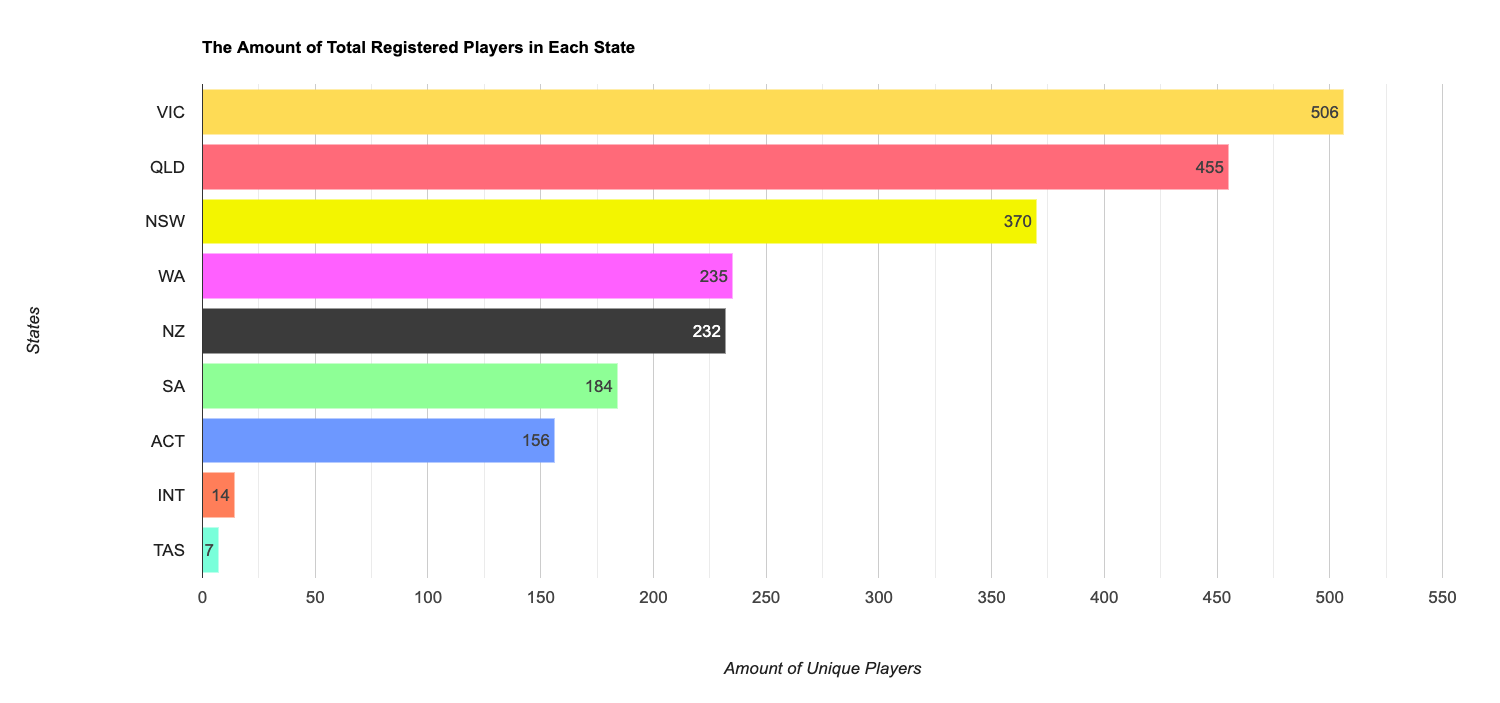
\includegraphics[scale=0.35]{/playerMatchGraphs/RegisteredPeople.png}}
	\caption{The Total Amount of Registered Players in Each State (2019)}
	\label{fig:figure1}
\end{figure}
The first graph that I wanted to display was that of unique players that had played in each state. From this graph, it is possible to see that Victoria (VIC) had the most registered players in 2019 while Tasmania (TAS) and International (INT) players have the smallest registered players, this may be due to the populus size of TAS and the lack of international competitors entering Australian tournaments. 

It's worth noting that New South Wales (NSW) should have a much larger registered playerbase due to its large population compared to all the other states. This however, does not seem to be the case, making it an outlier in the dataset. This could be due to a lack of tournaments held per week which can lead to a struggle in encouraging new players to join the gaming scene.

\newpage

\begin{figure}[!ht]
	\centerline{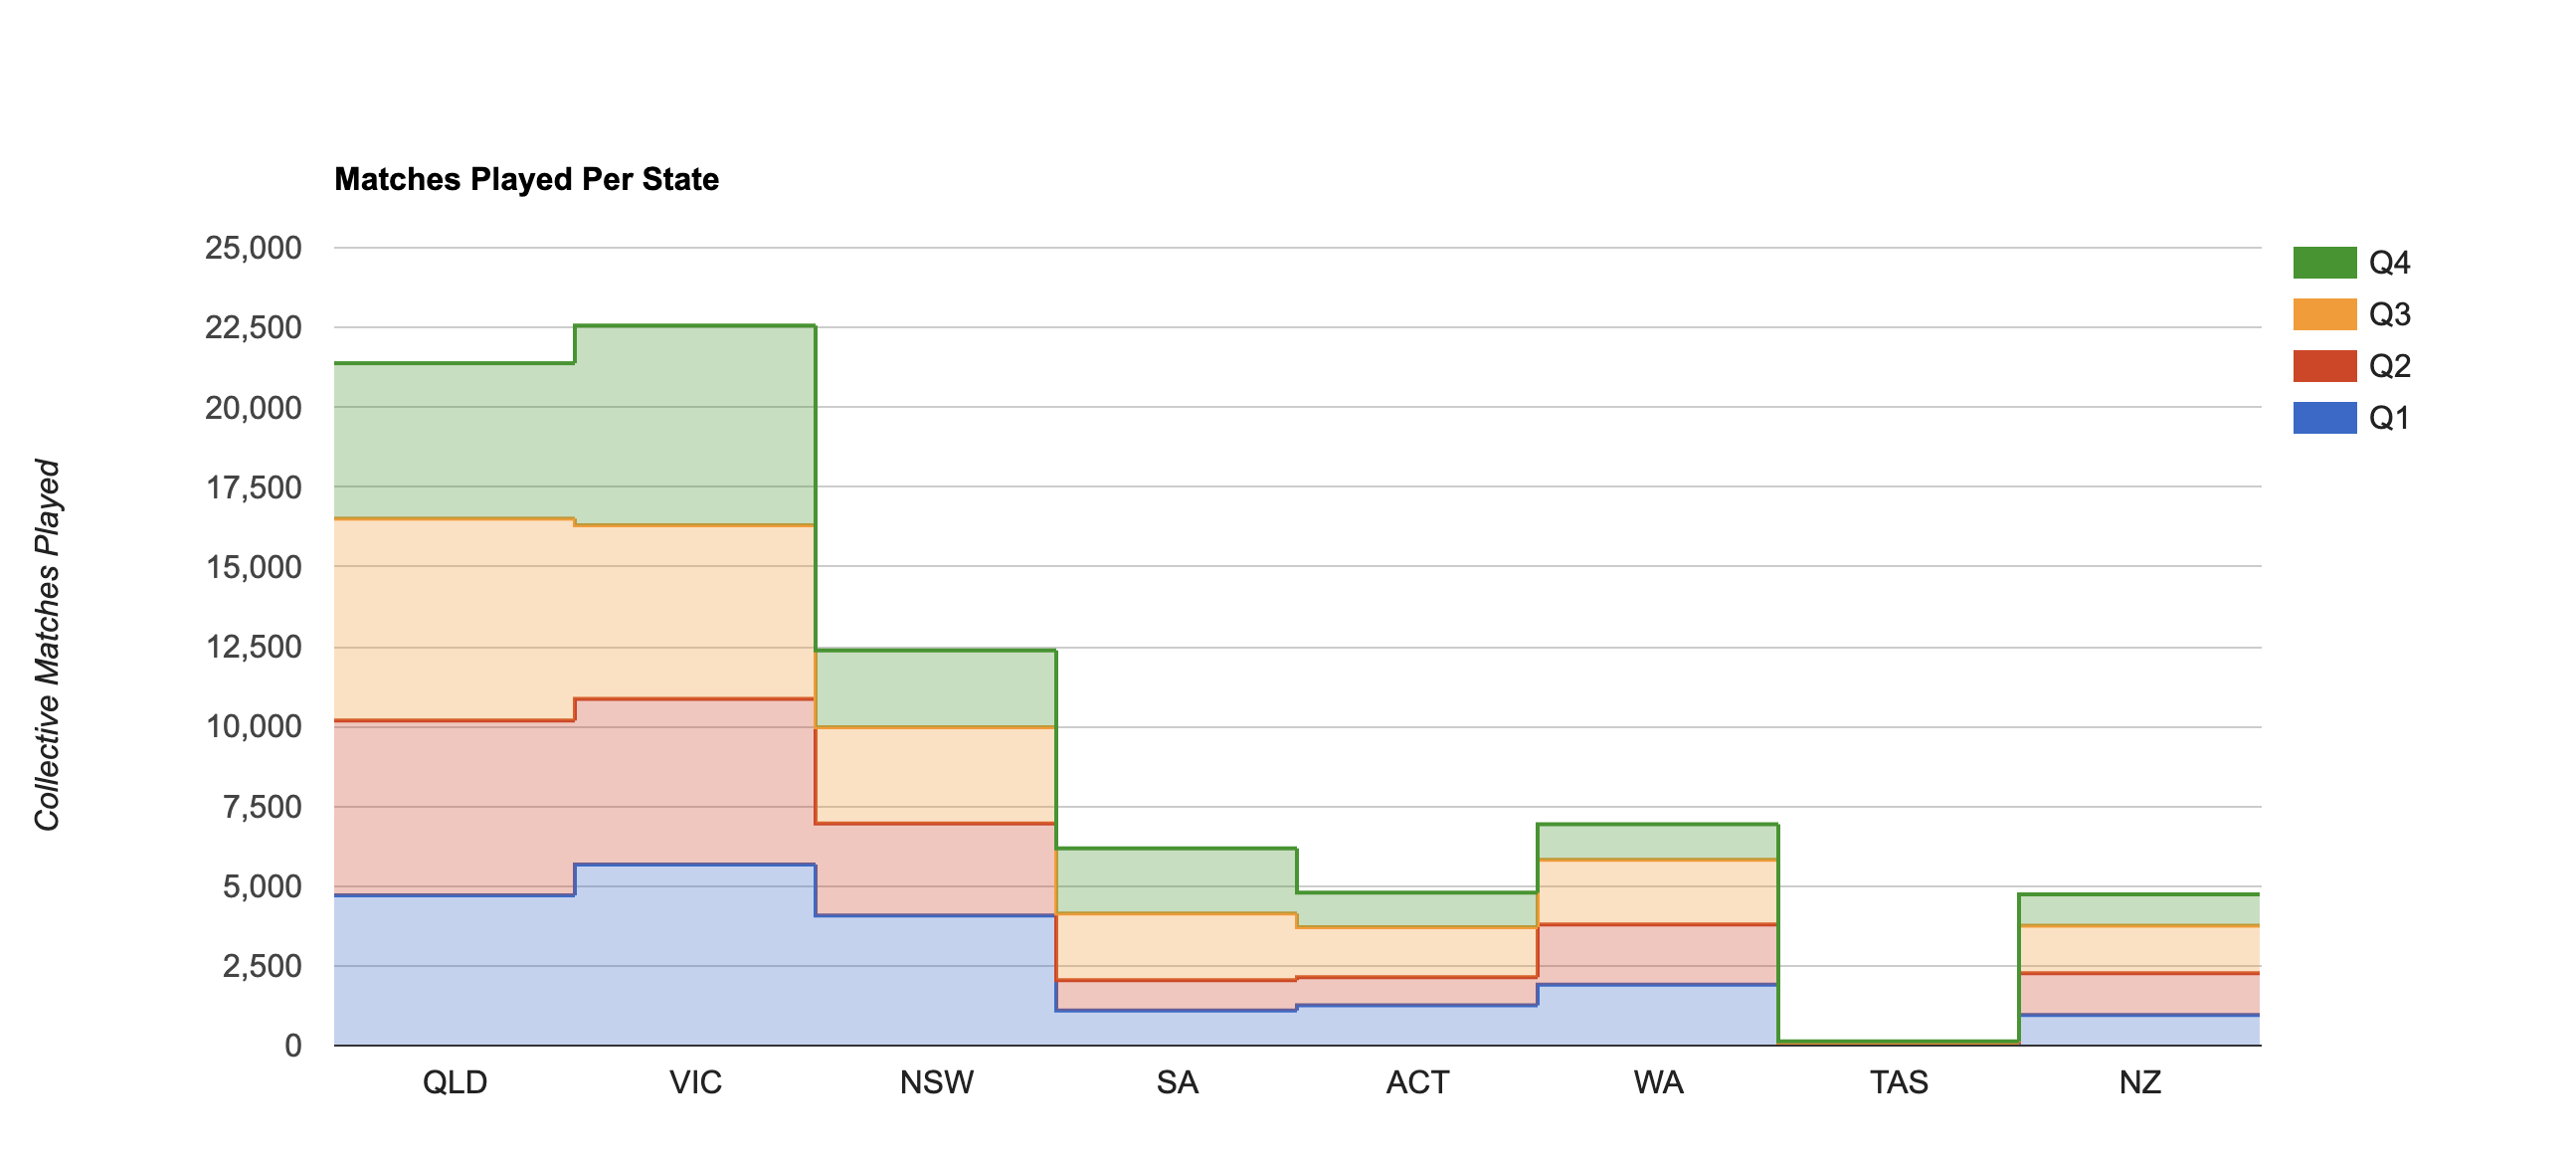
\includegraphics[scale=0.35]{/playerMatchGraphs/stepChart.png}}
	\caption{Step Graph Representing The Amount of Matches Played in Each State (2019)}
	\label{fig:figure2}
\end{figure}
Figure 2 shows the amount of matches that were played each quarter (Q) for each state. From the analysis of Figure 1, it is clear that the amount of players in a state can impact the total amount of matches played each quarter. As per Figure 1, VIC remains the state with the most amount of matches played across the year due to their large registered playerbase. 

Something not seen within Figure 1 that is seen in that of Figure 2 is that in the first quarter, NSW and QLD had a similar amount of matches played. This may have been due to the game's recent release as it came out in December which would've have brought many new players to start the year off with but as time went on, NSW players started to drop out of the scene and stop playing which resulted in less matches played in NSW for the rest of the year as the quarters following Q1 resulted in less matches played. One reason for NSW to have such a drop off in player base may be due to its community not being able to engage with new players properly unlike that of VIC and QLD's older communities which have been around since early 2010's, allowing them to be more experienced with new players.

It is also noticeable that TAS has almost no matches played in every quarter, each being around 27 for most of them which was also evident in Figure 1.

Since matches played isn't too much of a good measure of constant activity within a community. I decided to divide the total amount of matches by the players within each quarter to see if any further trends could be found.

\newpage
\begin{figure}[!ht]
	\centerline{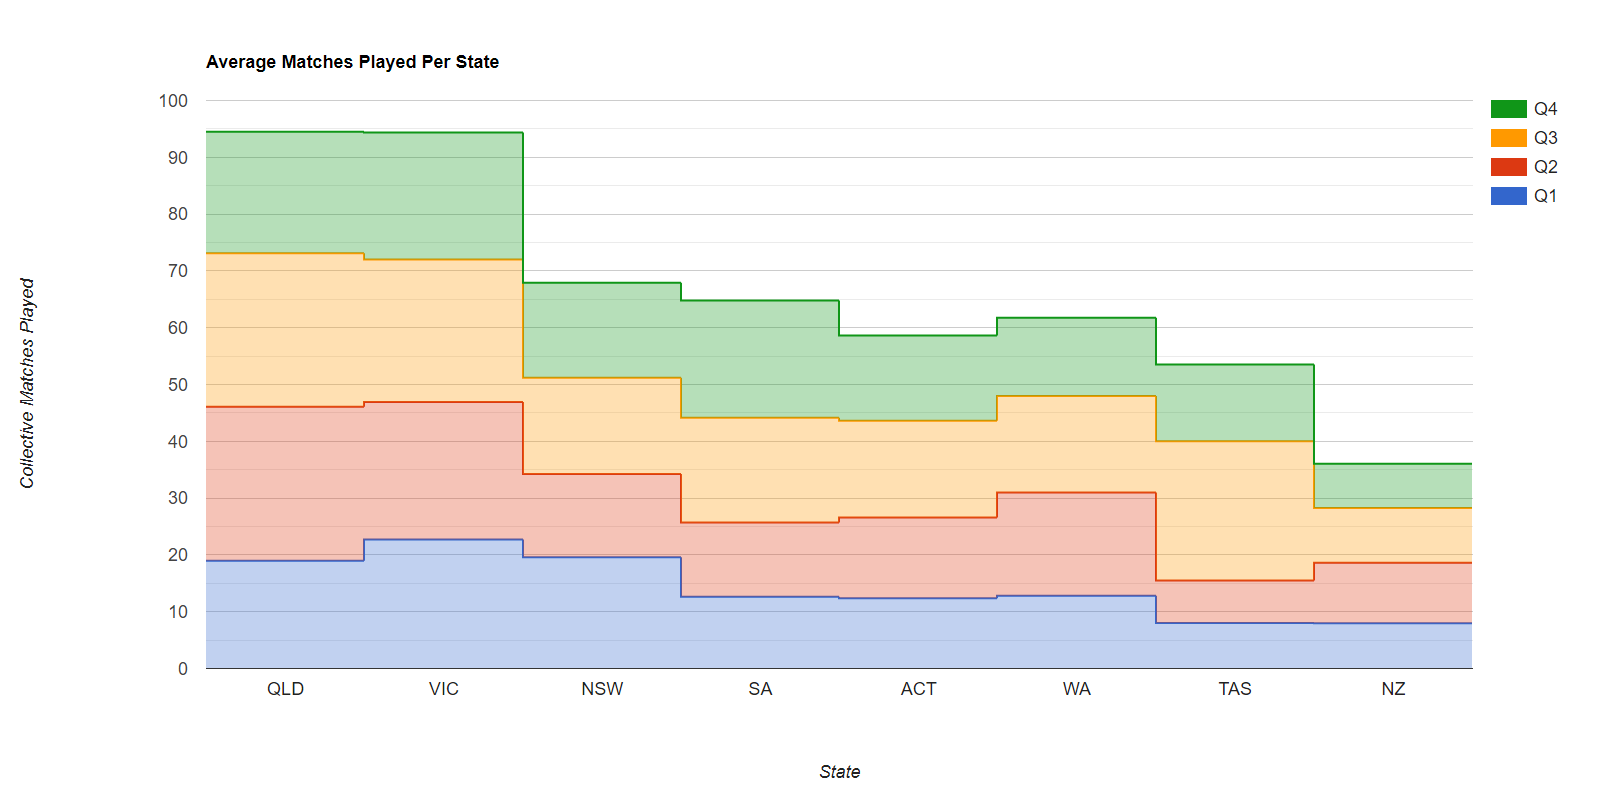
\includegraphics[scale=0.35]{/playerMatchGraphs/stepChartAverage.png}}
	\caption{Step Graph Representing The Average Amount of Matches Played in Each State (2019)}
	\label{fig:figure2}
\end{figure}

This graph differs very differently from the previous one. One noticeable difference being that of Tasmania's matches played. In the previous figure, TAS was barely visible in comparrison to other states, with the average calculation in play. It is possible to see that the TAS' competitive scene is rather active as each individual player is active. Similar to the other graph, New Zealand (NZ) has very steady data, with the amount of matches played and that of active players. From this, it is possible to assume that NZ players all have very similar attendence. This may be due to the fact that NZ does not have weekly tournaments but rather monthly ones.
\newpage
\subsection{Character Data Analysis}
When creating the bar graphs for this section of analysis. I decided to create an interactie bar graph which could show the character usage for each quarter per state and for the whole of Australia. Of course, this ended up with 32 different bar graphs to analyse... which I wasn't going to do. Instead, I will be analysing each quarter for the whole of Australia, there is a possibility that each graph will be looked at during the supplied presentation. It is also worth noting that due to the previous figures having a lack of non-average TAS and INT data, I have decided to take it out as they are outliers and are not good for individual analysis.

\begin{figure}[!ht]
	\centerline{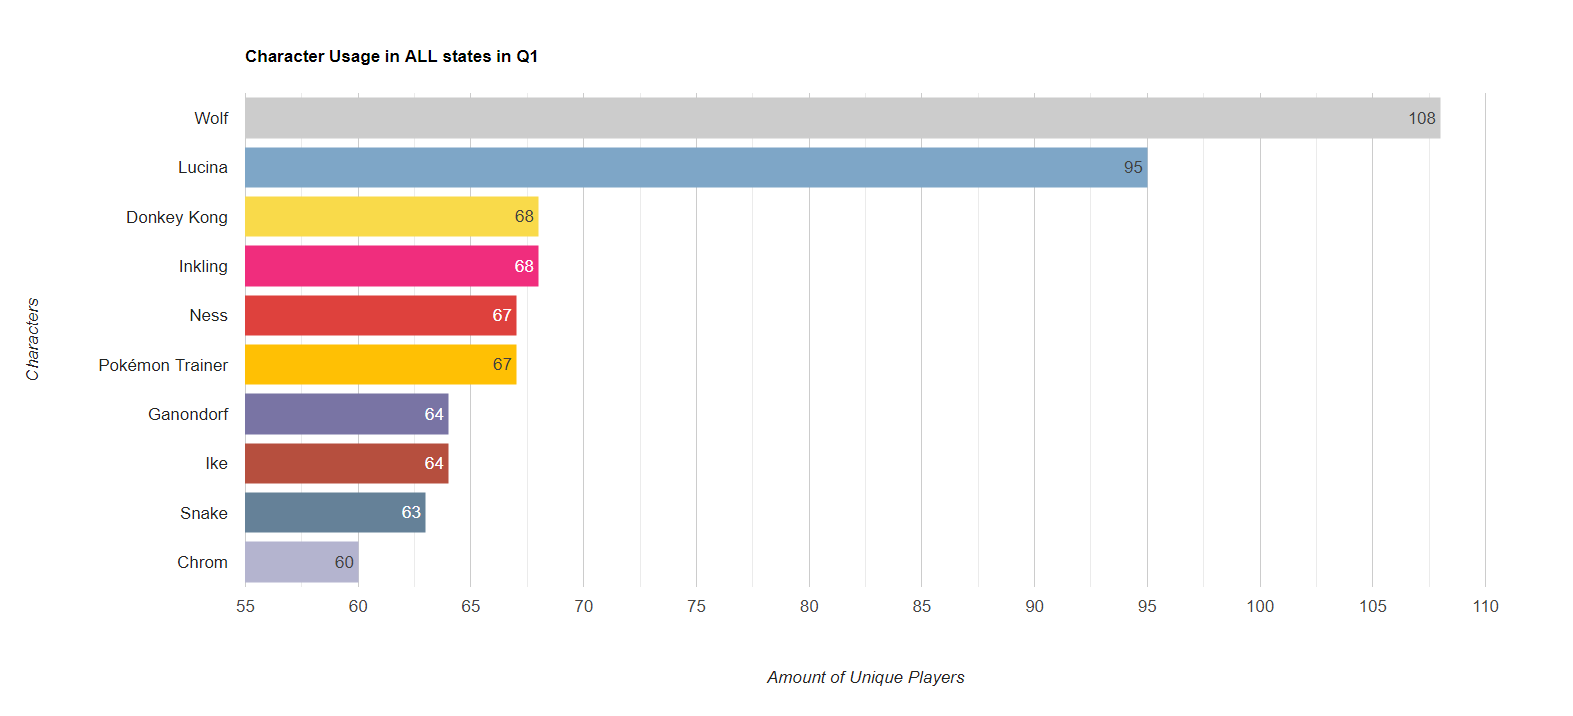
\includegraphics[scale=0.35]{/characterGraphs/Q1.png}}
	\caption{Character Usage in Australia, Q1 (2019)}
	\label{fig:figure2}
\end{figure}

Quarter 1 consisted of the time period spanning from the 1st of Jan to the 31st of March. During this time, no additional fighters were added to the game and it was relatively new. Due to the size of Smash Ultimate's character roster, many characters who did not appear in the previous game were added in game (Ultimate). This meant that fans who had missed older characters were finally able to play them again in this game. An example of this is Wolf, an older character who was not in the game before's roster. On the announcement of his return to the game, many fans were very eager to play him and explain his high usage within the first quarter. Similar to Wolf, Pokemon Trainer and Snake were also returning characters who were fan favourites which once again explain their popularity. 

Other characters such as Lucina were popular in previous games meaning when transitioning between games, players would choose characters they were more familiar with which would explain their popularity.

\newpage
\begin{figure}[!ht]
	\centerline{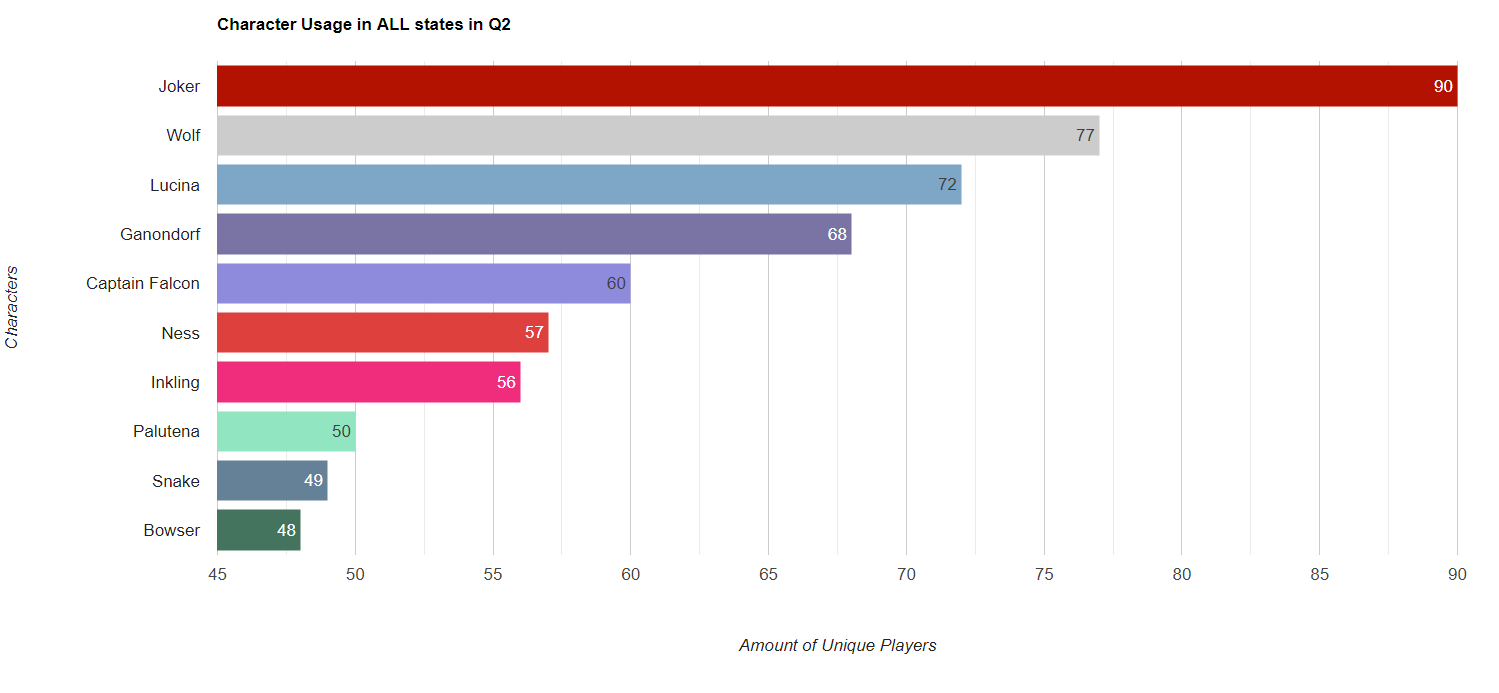
\includegraphics[scale=0.35]{/characterGraphs/Q2.png}}
	\caption{Character Usage in Australia, Q2 (2019)}
	\label{fig:figure2}
\end{figure}

Quarter 2 was when the first character (Joker) was added to the game. With the game still evolving and excitement revolving around the addition of the new character, players were eager to try out the new character. Although Joker was the most picked character for this quarter, there are less players who have chosen Joker than Wolf when comparing Q2 to Q1. This may be due to players dropping off

It is also worth noting that the two most played from Q1 (Wolf and Lucina) remain in the same order, meaning that players were more comfortable with them. Characters such as Palutena and Bowser have also appeared in this top 10 usage graph. This may be due to players branching out and experimenting with new characters.

\begin{figure}[!ht]
	\centerline{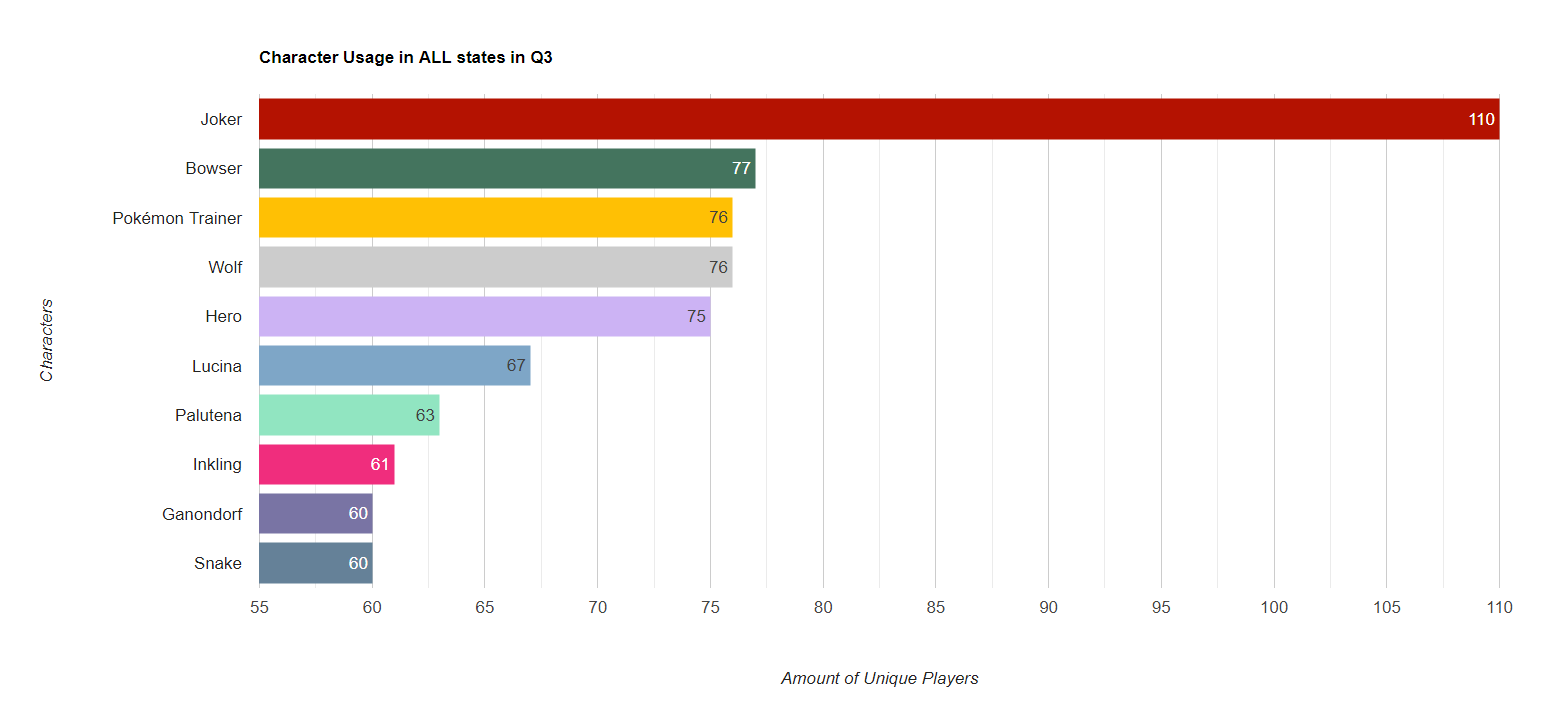
\includegraphics[scale=0.35]{/characterGraphs/Q3.png}}
	\caption{Character Usage in Australia, Q3 (2019)}
	\label{fig:figure2}
\end{figure}

Quarter 3 occured from the 1st of July to the 30th of September. During this time, another character (Hero) were added to the roster. Of course, players were eager to play him but his popularity was not enough to put him in the most played spot like Joker. This lack of popularity may be due to his moveset being controversial and based upon luck, resulting in some states banning the character and therefore, not allowing the whole of Australia to play him.

In this quarter, it is interesting to see that Joker is played significantly more than any other character, even overtaking Wolf's usage in Q1 (Figure 4). This may be due to the metagame (the way the game is played) finally evolving and players realising that Joker is a good character to play competitively. It is also worth noting that Bowser jumped from being the 10th most played in the country to the second most played within a quarter. 

\newpage
\begin{figure}[!ht]
	\centerline{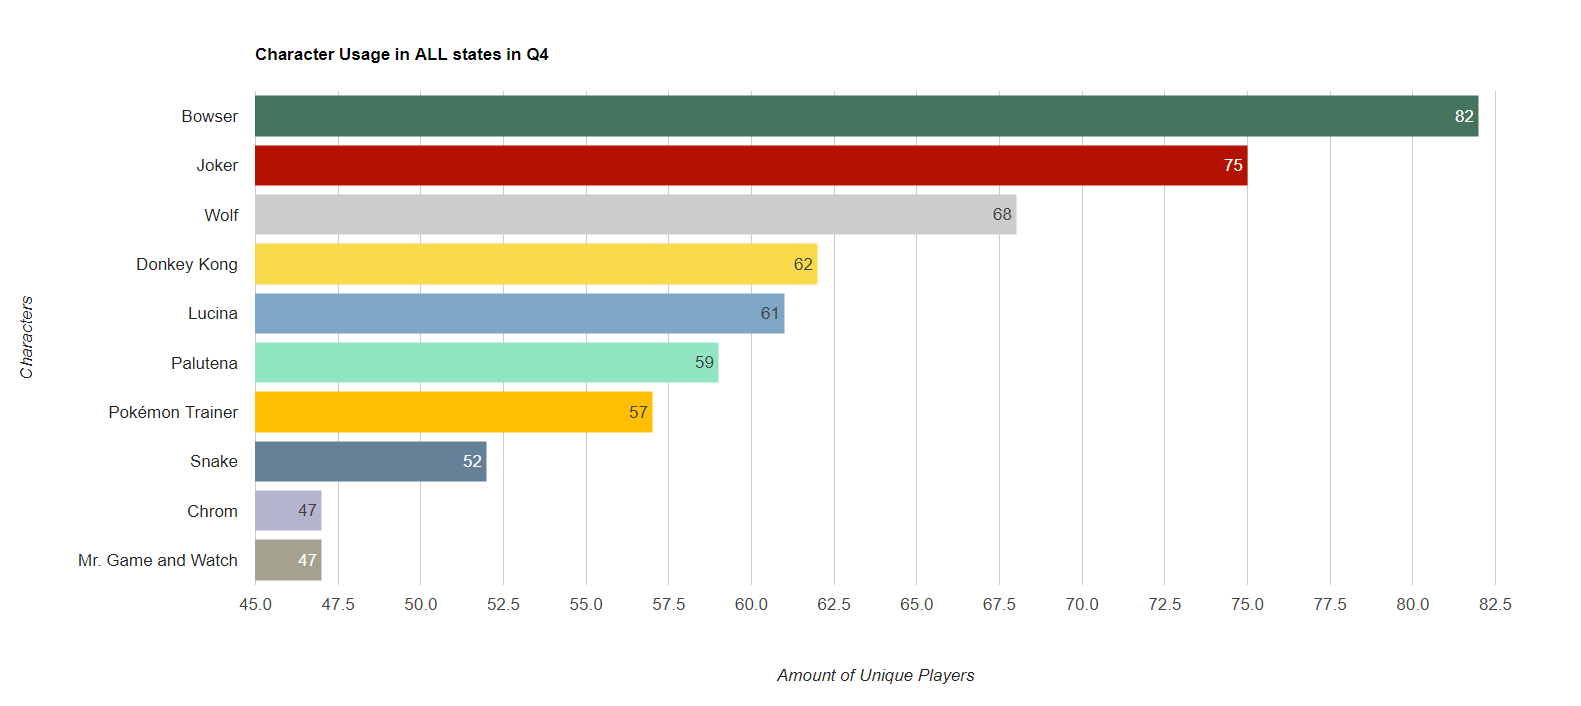
\includegraphics[scale=0.35]{/characterGraphs/Q4.png}}
	\caption{Character Usage in Australia, Q4 (2019)}
	\label{fig:figure2}
\end{figure}

Quarter 4 marks the end of the first year of competitive Smash Ultimate within Australia. Due to the previous two quarters, I expected this quarter to have Joker as the most played character but as you can see, he is not. Instead, Bowser is the most played. This may be due to players realising that Bowser's playstyle is more favoured for low level players which can allow them to win more games. Since there are is a decent amount of low level players, it would make sense that Bowser would be played more than Joker in low level. This may be a reason that Bowser was picked more than Joker in this quarter.

Mr. Game and Watch has also appeared on this graph and hasn't been seen within any other quarters. This may be due to a top player \href{https://liquipedia.net/smash/Maister}{Maister} beating some of the best players in the world and inspiring Australians to pick him up.

\newpage
\subsection{Elo Analysis}
Elo is that of skill rating within the smash community and acts as a way of seeing who is truly the best. When two players play a set against each other, they are to gain or lose elo based on an algorithm built into ausmash's backend. I however chose to look into purely elo gain as graphs could be more interesting as more elo is usually gained than lost within each state. 

\begin{figure}[!ht]
	\centerline{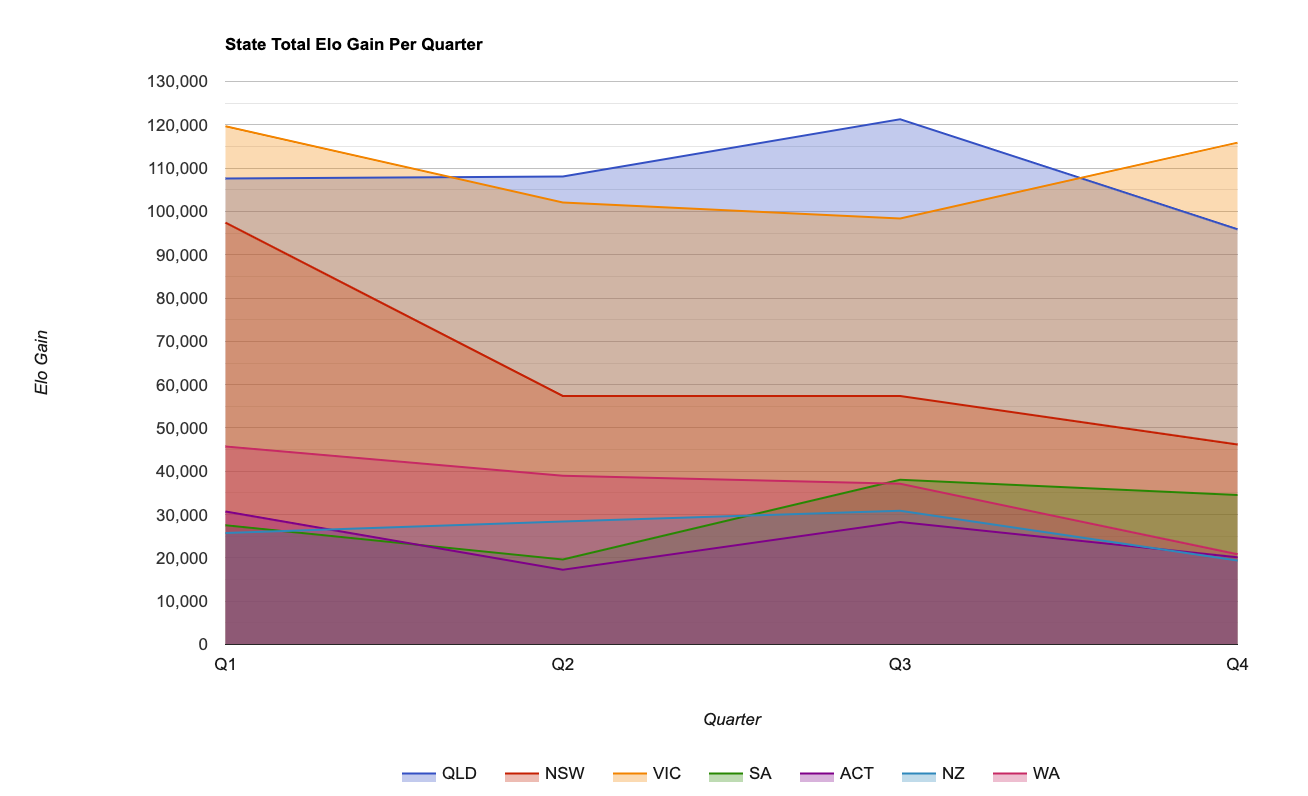
\includegraphics[scale=0.35]{/eloGraphs/EloGainLine.png}}
	\caption{Line Graph Representing Total Elo Gain within each State (2019)}
	\label{fig:figure2}
\end{figure}

The above line area graph show that of the fluctuating elo gain over each quarter of 2019. As seen in all previous graphs, QLD and VIC are always competing for the most elo/matches played due to their larger playerbases compared to other states. It's worth noting that VIC currently has the most top players residing in it which could result in more elo gain for players due to larger losses. Similar to what was seen in Figure 2, NSW has a large decline from Q1 to Q2 due to the player base greately decreasing which results in less elo being gained. It's also noteable that Q3 (July - September) has the largest difference between VIC and QLD. This was due to a lack of large events (majors) happening during this quarter. Only two majors were present during this quarter with one being in WA and the other being in QLD. This meant there were more opportunities for QLD players to gain elo as the tournament was local.

\newpage
Since elo gain is similar to that of player size, I decided to divide to total elo gain by the amount of unique players each quarter to get an average elo gain within each state.

\begin{figure}[!ht]
	\centerline{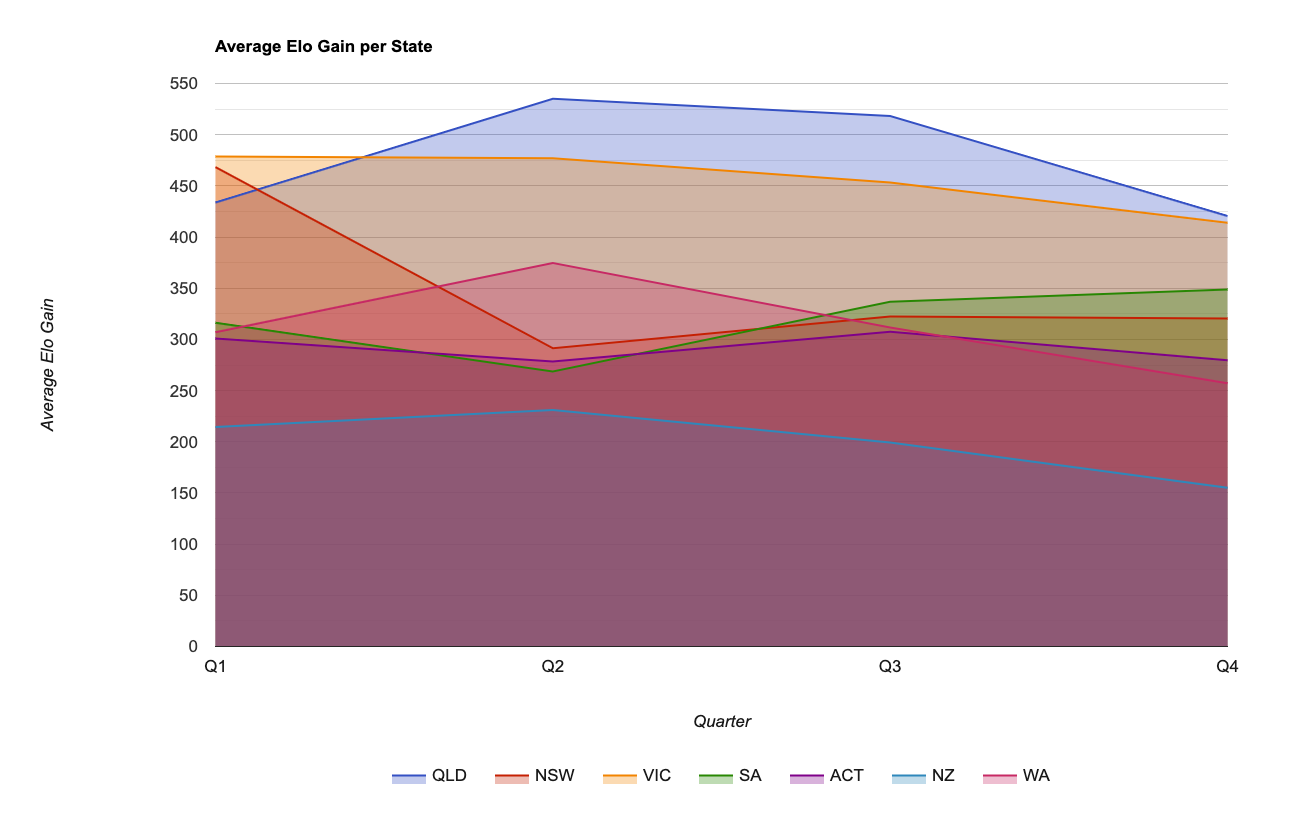
\includegraphics[scale=0.35]{/eloGraphs/AverageGainLine.png}}
	\caption{Line Graph Representing Average Elo Gain within each State (2019)}
	\label{fig:figure2}
\end{figure}

This change in from total to average elo gain can be drastically be seen. A main difference is that of the QLD vs VIC comparison and that of WA's spike in Q2. WA's spike particularly has not been seen in other graphs due to the player base size but due to the average calculation, it is easier to see the spike in Q2 where WA overtakes NSW in average elo gain. This could have been due to new characters being added to the game (Joker specifically) which could have allowed for players to perform better in tournaments.

From this figure alone, it is safe to assume that QLD had better players all around when compared to all other states in 2019. Although QLD was behind on average elo gain in Q1, as the game evolved, QLD was able to catchup and eventually have a better average elo gain.

As this was hard to analyse due to the line graph's colouring, I decided to use the same data points for a bar graph which can be seen in the figure below

\newpage
\begin{figure}[!ht]
	\centerline{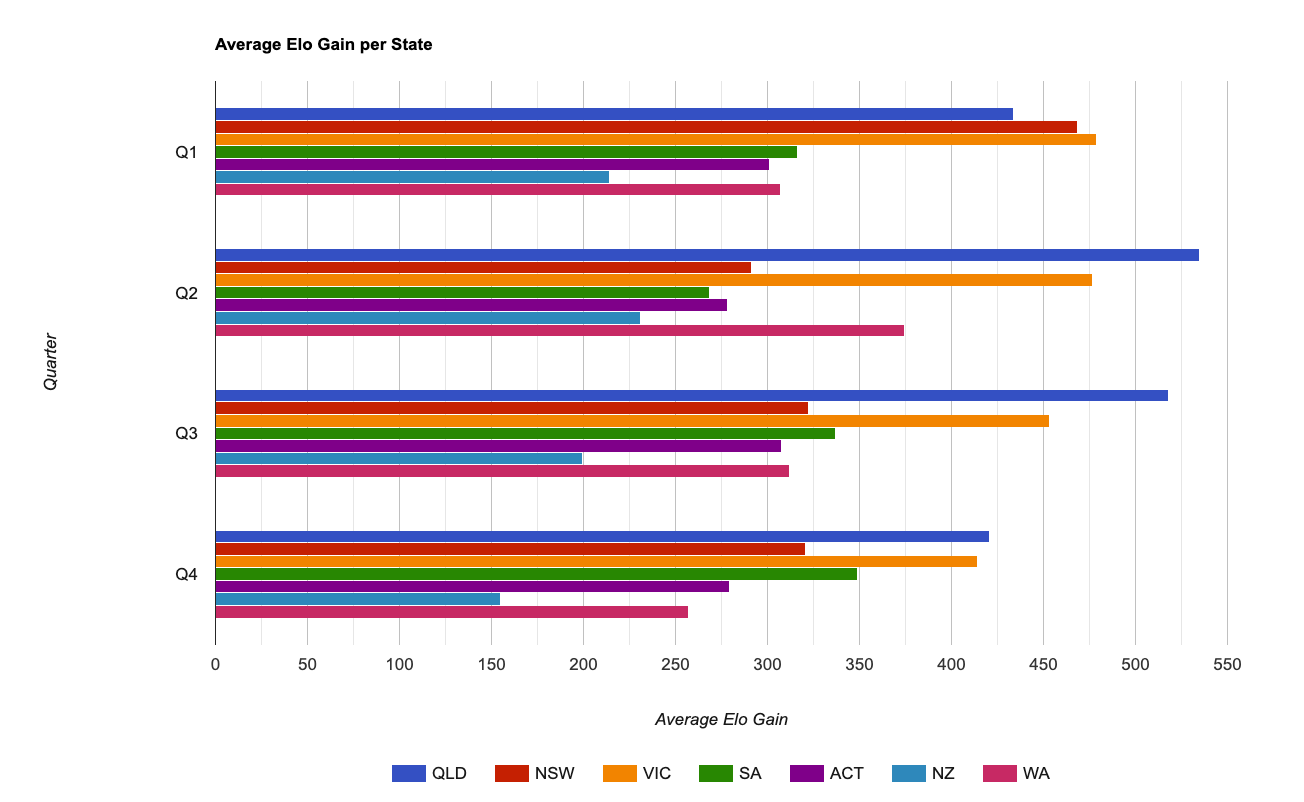
\includegraphics[scale=0.4]{/eloGraphs/AverageGainBar.png}}
	\caption{Bar Graph Representing Average Elo Gain within each State  (2019)}
	\label{fig:figure2}
\end{figure}

What can mainly be seen within this bar graph is similar to that of the previous line graph but with states being easier to see. As stated before, WA had a large spike in average elo gain in Q2. This can be seen more clearly in the bottom bar of each quarter as WA slowly increases and spikes in Q2 before slowly going down for Q3 and Q4. It's also easier to see that ACT had a very steady average elo gain with no fluctuations. This may have been due to the relatively small but active player base. 

Once again, it is safe to assume that QLD has better players all around due to its average elo gain across 2019 being much higher than other states for the majority of the year.

\newpage
\subsection{Multivariate Analysis}
Multivariate analysis of the data consists of combining more than three data points from previous sections and using it for further analysis. The two main sections that will be analysed will be:

\begin{itemize}
	\item Player Performance
	\item Character Performance
\end{itemize}

The reason that I have chosen to analyse performance with multivariate data is due to the fact that I wanted to display data on more than three axis as I am able to get a good indicator of how different players and characters perform.

\subsubsection{Player Performance}
Player performance graphs used the axis of elo gain, the amount of registered players and later on, quarters and states. In later scatterplots, you will see the data becomes easier to read as I add labels and colours to them.

\begin{figure}[!ht]
	\centerline{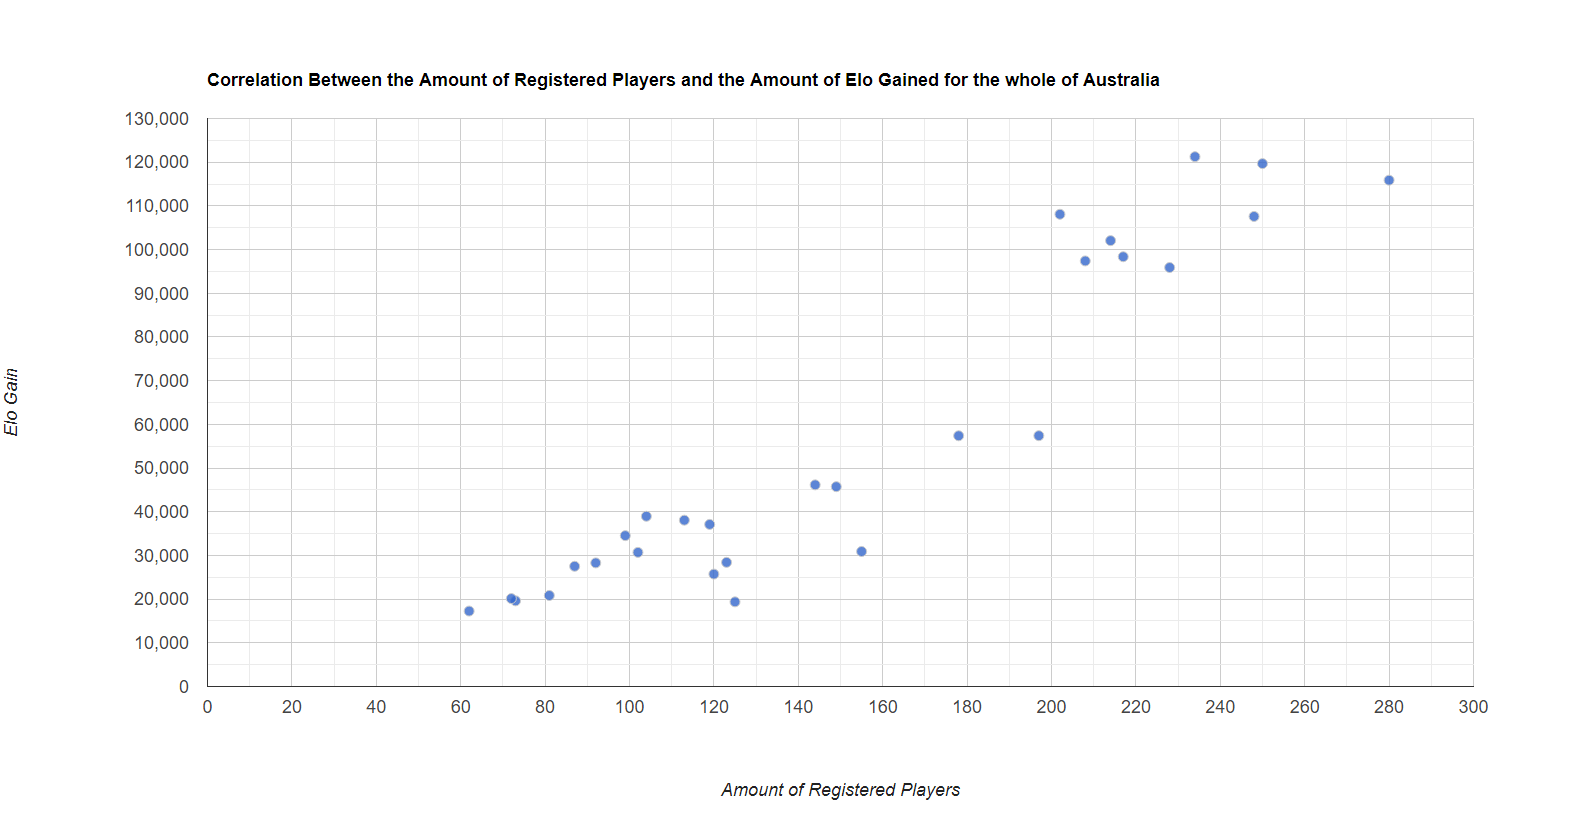
\includegraphics[scale=0.4]{/mixed/scatterPlotAllYear.png}}
	\caption{Player Performance in 2019}
	\label{fig:figure11}
\end{figure}
Figure 11 demonstrates a base graph with no colour. The point of this graph was to demonstrate and show the trend that the more registered players there are, the higher the elo gain for the players is. Each dot/point in this graph is representative of a state in a quarter which is looked at a little bit later but for now I wanted to show that this trend exists before adding more data points to it.

\newpage
\begin{figure}[!ht]
	\centerline{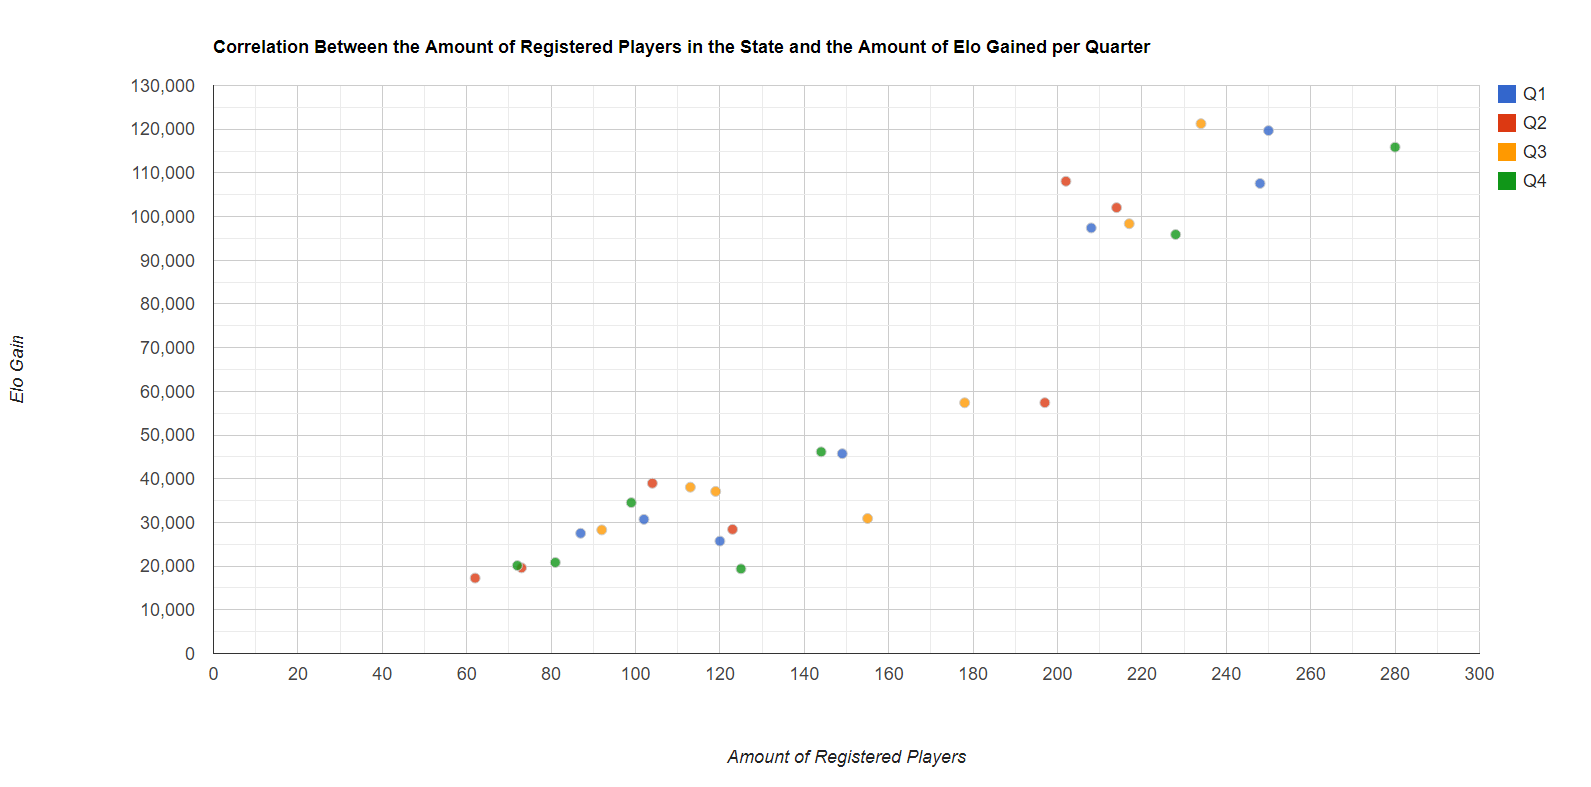
\includegraphics[scale=0.4]{/mixed/scatterPlotQuartersNoLabel.png}}
	\caption{Quarters and Player Performance (2019)}
	\label{fig:figure12}
\end{figure}

Figure 12 shows the addition of quarters to the graph. What would be expected from this graph would be that of Q1 having the highest registered players and hence, the most elo gain. This is evident as the majority of the dots in the top right corner which represent the highest of both axis belong to that of Q1. It's interesting that the rest of the quarters have an even distribution in this top corner. 

Q4 also had the most players for a state and is much larger when compared to other data points while Q2 for a state had the least amount of players recorded. For the first point, it is expected that this state would be a larger region (e.g. QLD or VIC) while the smaller point would be that of a smaller region (e.g. ACT, SA).

It's also worth noting that a state's performance in Q3 had the highest elo gain. This quarter was around the time of a QLD major so it would be expected that this dot is representative of QLD. 

In the next figure, states were labelled in the scatterplot.

\newpage
\begin{figure}[!ht]
	\centerline{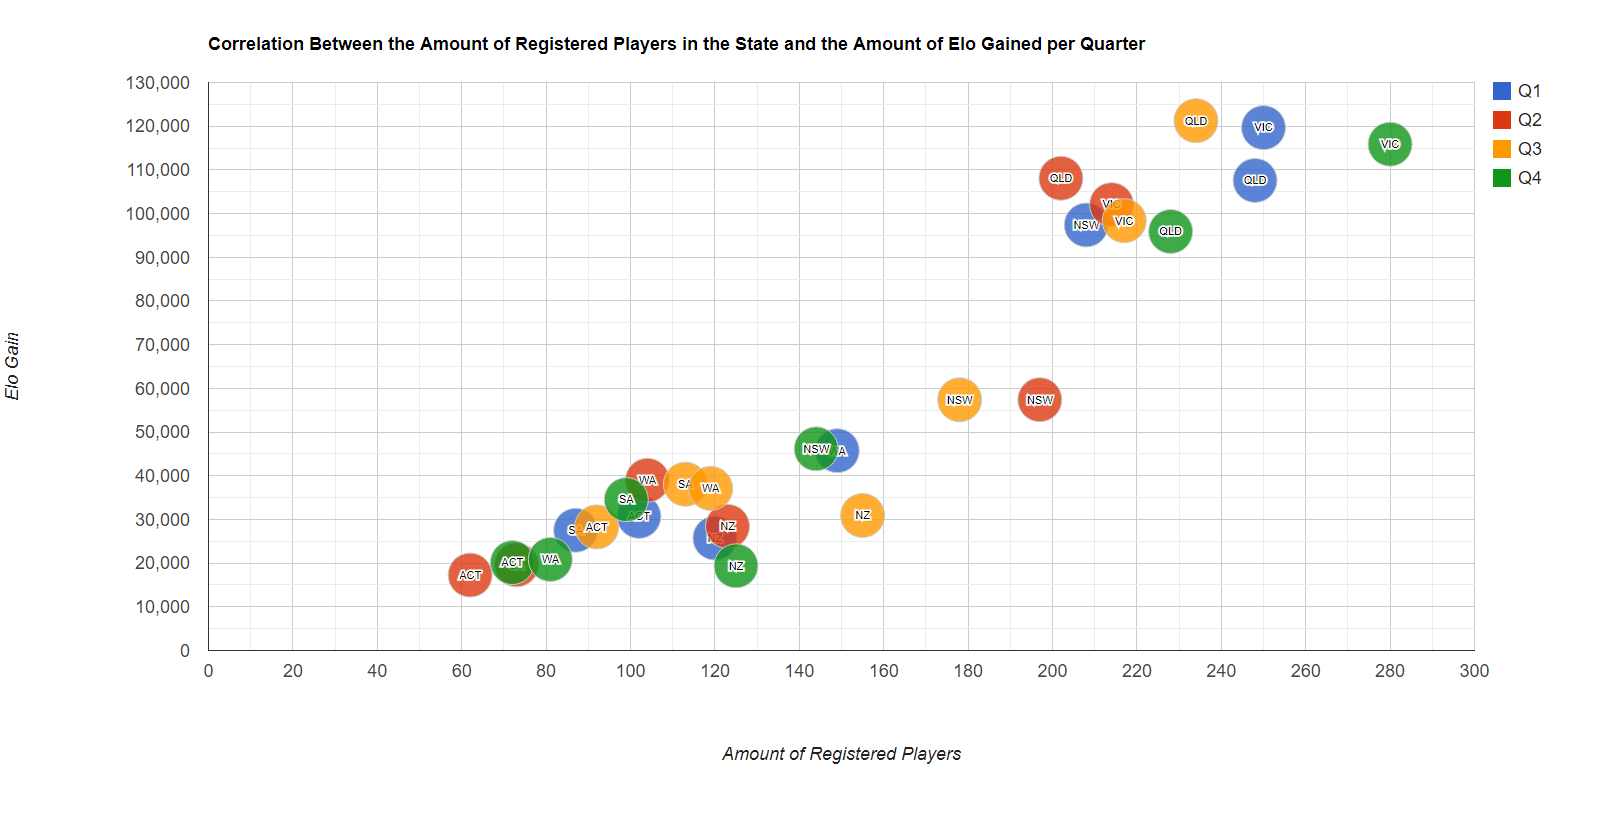
\includegraphics[scale=0.4]{/mixed/scatterPlotQuartersLabels.png}}
	\caption{Quarters and Player Performance in States (2019)}
	\label{fig:figure13}
\end{figure}

In Figure 13, you can see the states added to the quarter labels. It's once again possible to assume that from the data that the more dominant states are that of VIC and QLD once again. 

It was pointed out in the previous figure that a state in Q3 had the highest elo gain within the whole year and out of all the states. This lined up with my prediction of it being QLD due to the major event. This is also notaeble as this is the largest gap in elo gain between QLD and VIC but is still less than VIC and QLD's elo gain gap in Q4.

As per previous figures, specifically in that of the elo gain analysis section. NSW can once again be seen signifcantly dropping off in elo gain after Q1. 

One point that can be seen here that wasn't evident in previous figures is that of NZ in comparrison to SA's Q4 performance. While the region had larger player base than SA, NZ underperformed and did not gain more elo than SA which stands as an outlier. 

Another thing worth noting is that QLD in Q2 had better performing players than VIC. This can be seen as QLD in Q2 had more elo gain than VIC in Q2 despite having less players.

\newpage
\subsubsection{Character Performance}
Character performance looks at quarters and 2019 as a whole. It aims to analyse and look into which characters were popular at the time and had the most elo gain. This would allow me to find the best performing characters within 2019.

\section{Extras}


\end{document}